\documentclass[12pt]{article}
\usepackage[utf8]{inputenc}
\usepackage{csquotes}
\usepackage[ngerman]{babel}
\usepackage[backend=biber, style=apa, sorting=nty]{biblatex}
\renewcommand*{\bibfont}{\small}
\addbibresource{citation.bib}
\usepackage[T1]{fontenc}
\usepackage[top=2cm,left=3cm,right=2cm,bottom=2cm]{geometry}
\usepackage[parfill]{parskip}
\usepackage[font=normalsize]{caption}
\usepackage{hyperref}
\usepackage{multirow}
\usepackage{amsmath}
\usepackage{amssymb}
%% From HAW-Template
\usepackage{setspace}
\usepackage{listings}
\usepackage{graphicx} %% Important for including pictures
\graphicspath{{./images/}}
%% define colors in article
\usepackage{xcolor}
\definecolor{arsenic}{rgb}{0.23, 0.27, 0.29}
\definecolor{smokyblack}{rgb}{0.06, 0.05, 0.03}
\definecolor{coolblack}{rgb}{0.0, 0.18, 0.39}
\definecolor{mistyrose}{rgb}{1.0, 0.89, 0.88}
\hypersetup{
  colorlinks=true,
  linkcolor=black,
  filecolor=cyan,
  urlcolor=coolblack,
  citecolor=black,
}

%% \linespread{1.25} %% Paragraphs 1.5 lineheight
\onehalfspacing

%% \setmainfont{Arial}
\usepackage{uarial}
\renewcommand{\familydefault}{\sfdefault}

%% to set size of headings as normalsize 12pt
\usepackage{sectsty}
\sectionfont{\normalsize}
\subsectionfont{\normalsize}

%% to change space of headings to 0
\usepackage{titlesec}
\titlespacing*{\section}
{0pt}{12pt}{6pt}
\titlespacing*{\subsection}
{0pt}{6pt}{6pt}
\titlespacing*{\subsubsection}
{0pt}{6pt}{6pt}

%% set headers 
\usepackage{fancyhdr}
\pagestyle{fancy}
\fancyhf{}
\rhead{\textit{\footnotesize{Duy Nguyen. 2359864}}}
\rfoot{\thepage}
%% change paragraph margins
\usepackage{changepage}
\usepackage{subcaption}
\title{Vorstellung der Drucksensoren}
\author{Duy Nguyen}

%% Begin document
\begin{document}
\pagestyle{empty}
\color{smokyblack}

\setlength{\parskip}{1ex}
\begin{table}[t]
  \begin{center}
    \begin{tabular}{p{0.7\textwidth}r}
      \small{HAW-Hamburg} & \multirow{4}{*}{
\includegraphics[width=4.6cm]{haw-logo}} \\
      \small{Vorlesung Messtechnik} &  \\
      \small{Sommersemester 2021} & \\
      \small{Prof. Dr. Carsten Frank} & 
    \end{tabular} 
  \end{center}
\end{table}

\vspace{2cm}

\textsf{\textit{\Large{Hausarbeit}}}

\color{arsenic}
\textsf{\textbf{\huge{Drucksensoren}}}
\setlength{\parskip}{0.8em}
\color{smokyblack}
%% Add abstract paragraph

\begin{adjustwidth}{3em}{0pt}
\begin{flushleft}
	\textit{Duy Nguyen} 

  \vspace{-12pt}

  \textit{\footnotesize{Feinstaubsgruppe: Duy Nguyen, Ferris Fensky, Dennis Dick}}
\end{flushleft}
\end{adjustwidth}

\tableofcontents
\newpage
\listoffigures
\addcontentsline{toc}{section}{Abbildungsverzeichnis}
\listoftables
\addcontentsline{toc}{section}{Tabellenverzeichnis}

%% Uncomment these lines to input manually list of abbreviations as IV from external file
%% \input{abbreviationpage}
%% \addcontentsline{toc}{section}{List of abbreviations}

\newpage
\pagestyle{fancy}
\section{Drucksensoren}
\label{sec:drucksensoren}
In diesem Projekt ist möglich, dass einen Luftdrucksensor gebraucht wird. Dafür brauchen wir einen ziemlich empfindlichen Sensor. Der Messbereich liegt zwischen 925hPa und 1070hPa, da die Messstation sich unter normaler Atmösphärebedingung gestellt wird (wetter.de). Daher ist 2 unterschiedliche Drucksensoren vorgestellt: Halbleiterdehnungsmessstreifen (Halbleiter-DMS) und piezoelektrische Dehnungssensoren. 

\subsection{Halbleiterdehnungsmessstreifen}
\subsubsection{Funktionsprinzip}
Dehnungsmessstreifen basieren vor allem auf geometrieabhängiger Widerstandsänderung (bei Metall-DMS) oder Anwendung des piezoresistiven Effekts (Halbleiter-DMS). Wird ein DMS gedehnt, nimmt die Länge des Leiters zu und dessen Querschnitt wird kleiner, daher steigt deren Widerstand an. Der k-Faktor zeigt die Empfindlichkeit des Dehnungsmessstreifens und beträgt bei Metall-DMS einen Wert von 2. Mit Halbleiter gemachte DMS beruhen auf piezoresistiven Effekt, dass die mechanische Deformation des Siliziumskristalls die mittlere Beweglichkeit der Ladungsträger und damit den elektrischen Widerstand ändert (\cite{Buttgenbach.2016}). Im Gegensatz haben Halbleiter-DMS größere (und nicht lineare) Temperaturempfindlichkeit im Vergleich mit Metall-DMS. (\cite{Heimann.}) Halbleiter-DMS wird im Prinzip auch  wie normale Metall-DMS auf einem Objekt drauf geklebt. Wegen ihres $SiO_2$ Kristalls haben Halbleiter-DMS hohe Empfindlichkeit und auch hohe $k$-Wert. Bei p-dotierte Halbleiter-DMS kann $k$ über 150 groß sein. Bei n-dotierte Halbleiter-DMS trägt k einen Wert < -100. 
Es wird häufig aufgetreten neben der Messung von Dehnungen, dass die DMSs als Sensorelement in Kraftmessdosen zur indirekten Kraftmessung eingesetzt. Da befindet sich ein Hohlzylinder, wobei die einwirkende Kraft F und die Dehnung an DMS transportiert werden. Die Vollbrückenschaltung dazu garantiert eine hohe Empfindlichkeit und sehr gute Temperaturkompensation. (\cite{Parthier.2006}). Aber eine gute Lösung könnte auch, dass daneben die Temperatur gleichzeitig gemisst wird, eine Temperaturkoeffizient wurde ermittelt und dann wird als Korrektursfaktor an Druckmesswerten angewendet. (\cite{Siemens.2021})

\subsubsection{Beispiel piezoresistiver Drucksensor}
\begin{figure}[h]
  \centering
  \label{fig:bcmsensor}
  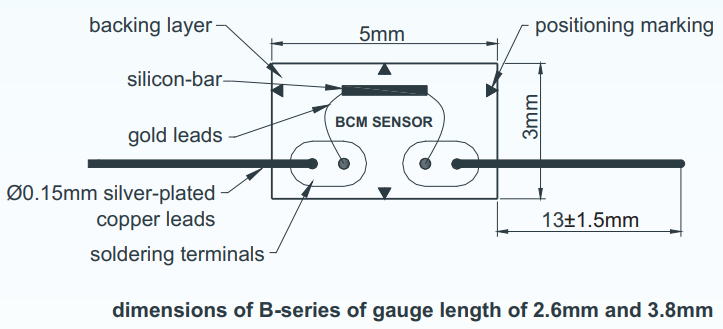
\includegraphics[width=0.7\textwidth]{halbleiterdms}
  \caption{Aufbau Halbleiter-DMS mit modifiziertem Polymidharz (\cite{Wu.1992})}
\end{figure}

Damit es an allen Richtungen messbar ist, nutzt man die Anordnung in 2 Richtungen mit vier Halbleiter-DMS und eine Vollbrücke Wheat-stone Brücke Schaltung. 
\begin{figure}[h!]
  \centering
  \begin{subfigure}[b]{0.4\linewidth}
    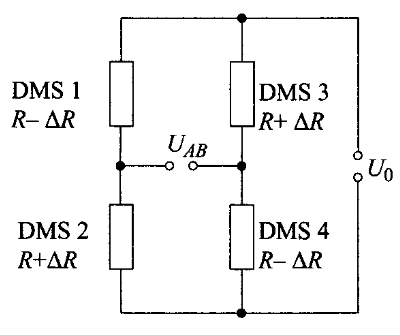
\includegraphics[width=\linewidth]{vollbruecke}
    \caption{Wheat-stone Brücke Schaltung (\cite{Parthier.2006})}
  \end{subfigure}
  \begin{subfigure}[b]{0.4\linewidth}
    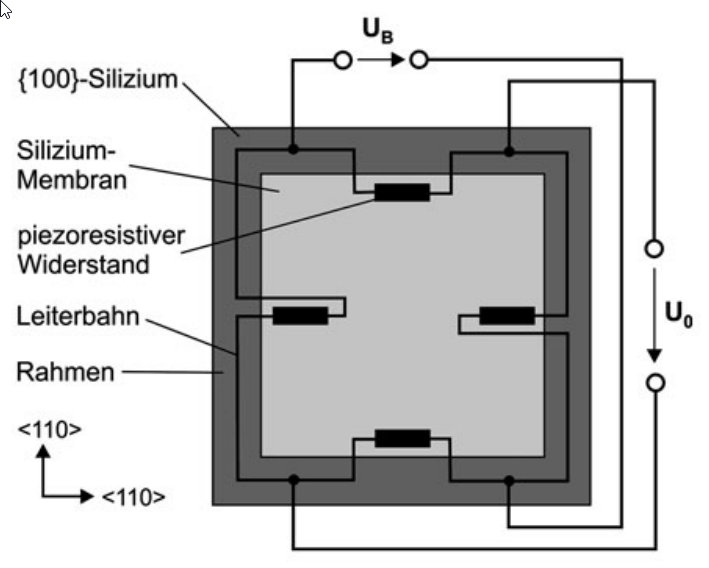
\includegraphics[width=\linewidth]{anordnungpiezoresistiv}
    \caption{Anordnung von Piezowiderständen auf einer quadratischen Membran (\cite{Buttgenbach.2016})}
  \end{subfigure}
  \caption{Anordnung von Piezowiderständen in Betrieb}
  \label{fig:anordnung}
\end{figure}

Werden 2 gegenliegende Piezowiderstände gedehnt, gibt es Widerstandsänderung und die Spannungsausgang $U_{AB}$ wird hergestellt und berechnet durch Formel (\ref{uab}):
\begin{equation}\label{uab}
    U_{AB} = U_0 \cdot \frac{\Delta R}{R} = U_0 \cdot \epsilon \cdot k
\end{equation} 

Hier wurde der piezoresistive Widerstand KPY43-A gewählt. Datenblatt (\cite{Siemens.2021})

\begin{figure}[h!]
  \centering
  \label{fig:kpy43a}
  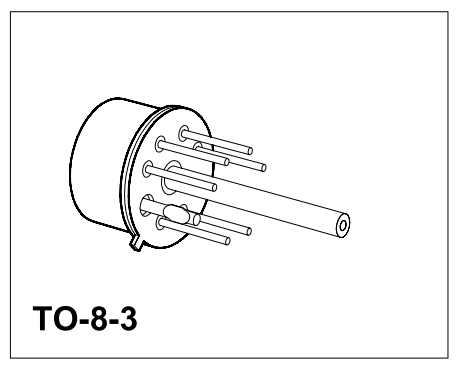
\includegraphics[width=0.3\textwidth]{kpy43a}
  \caption{Silicon Piezoresistive Absolute Pressure Sensor KPY43-A (\cite{Siemens.2021})}
\end{figure}

Eine Schaltung ist dafür geeignet: 
  
\begin{figure}[h]
  \centering
  \label{fig:piezoschaltung}
  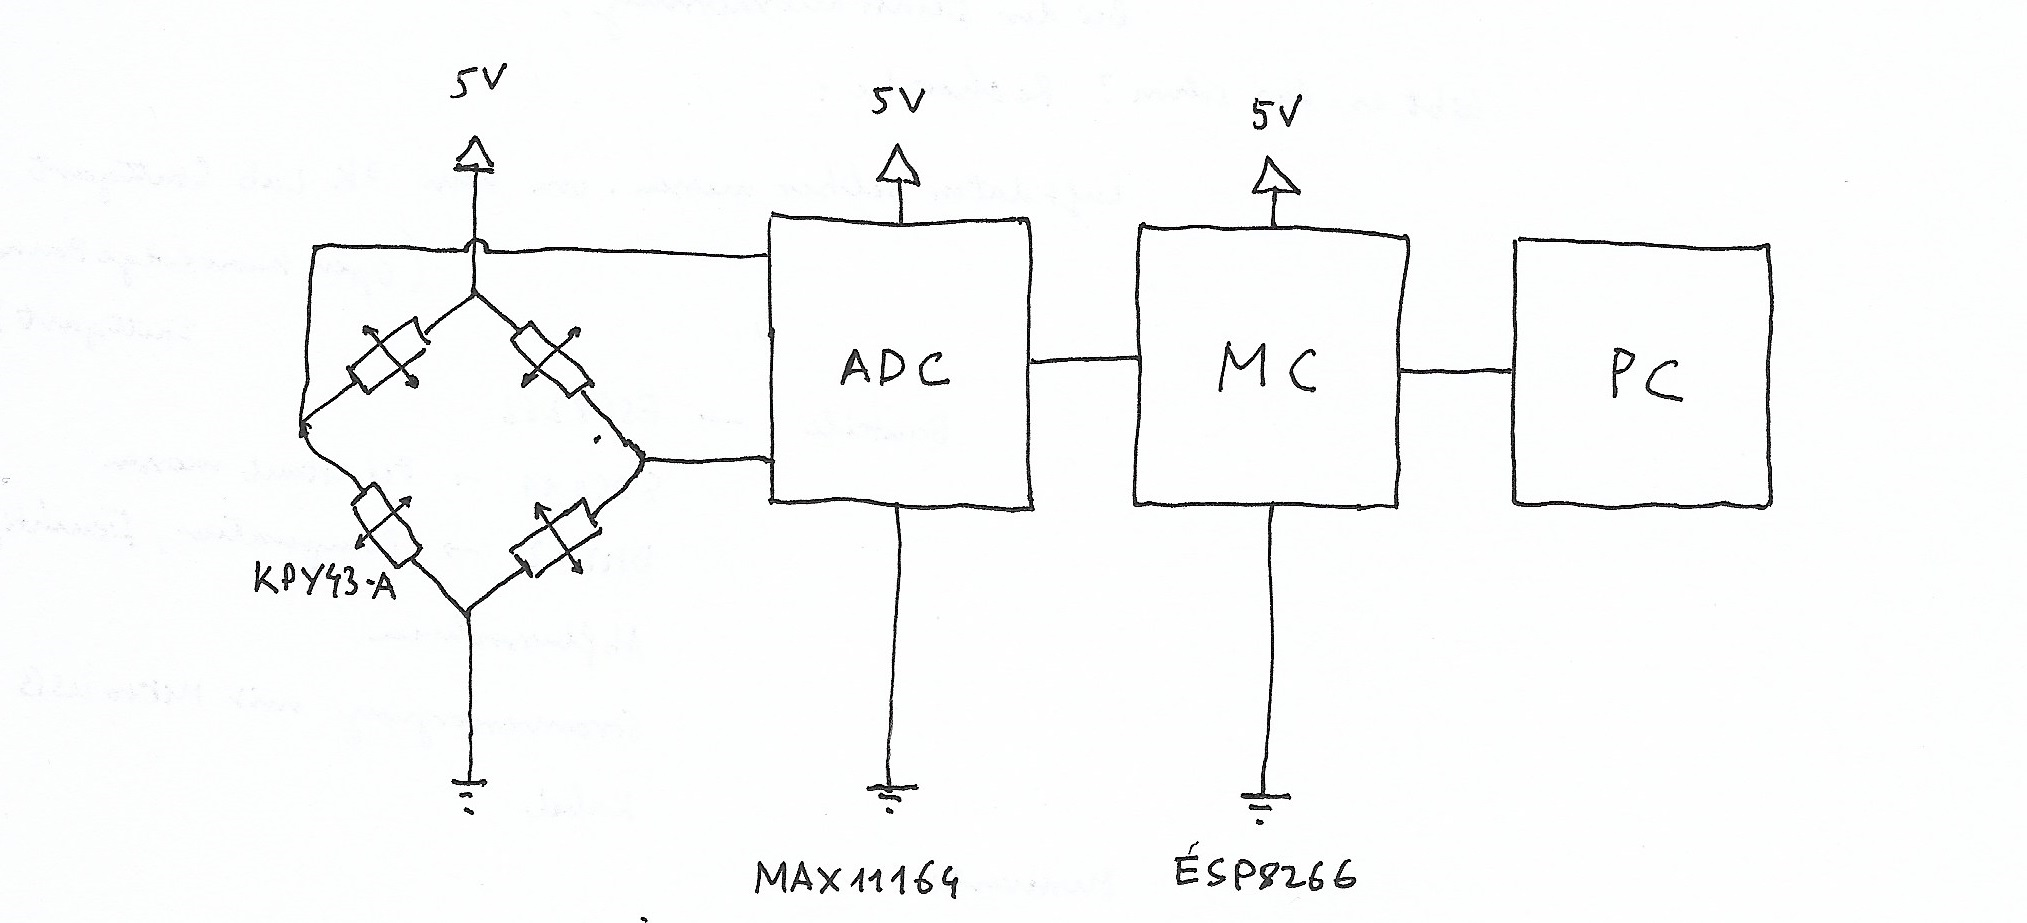
\includegraphics[width=0.8\textwidth]{schaltungpiezoresistiv}
  \caption{Schaltung des piezoresistiven Drucksensor KPY43-A}
\end{figure}

\begin{table}[h]
  \caption{\normalsize{Gewählte Parameter zur Berechnung der Auflösung des piezoresistiven Drucksensor}}
  \begin{center}
    \begin{tabular}{r|l}
    Parameter & Wert \\
    \hline
    Widerstand $R_{KPY43-A}$ & 120 $\Omega$ \\
    Maximal zulässige Dehnung $\epsilon_{max}$  & $5.10^{-3}$ m/m \\
    k-Faktor & 100 \\
    $V_{IN}$ & 5V \\
    \end{tabular} 
  \end{center}
\end{table}

Mit der maximal zulässige Dehnung $\epsilon_{max}$, k und R haben wir aus der Formel \ref{uab}: 

\begin{center}
$\Delta R = \epsilon_{max} \cdot k \cdot R = 100 \cdot 5 \cdot 10^{-3} m/m \cdot 120 = 60 \Omega$ 
$U_{AB} = U_{IN_ADC} = \frac{\Delta R}{R} \cdot U_0 = \frac{60}{120} \cdot 5 = 2.5V$
\end{center}

Die Schaltung sieht jetzt so aus mit den Werten: 
\begin{figure}[h!]
  \centering
  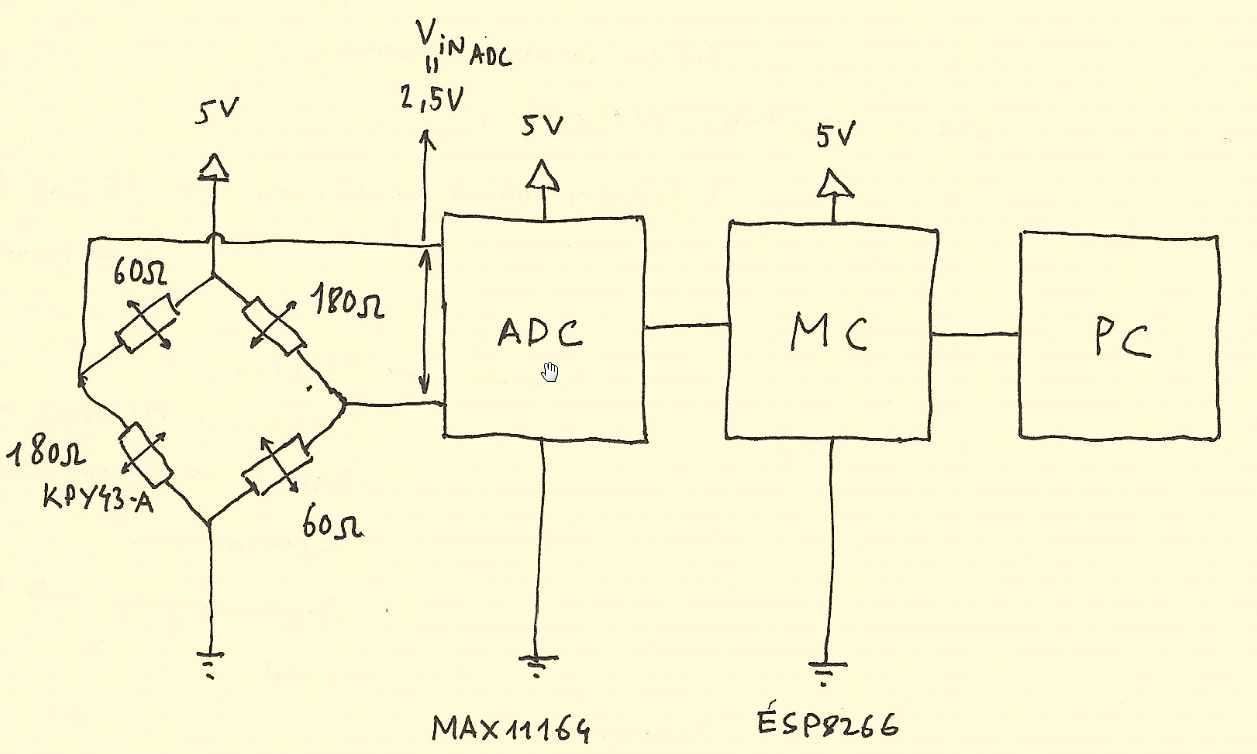
\includegraphics[width=0.75\textwidth]{schaltungpiezoresistivmitwert}
  \caption{Schaltung des piezoresistiven Drucksensor KPY43-A mit berechneten Widerstände}
\end{figure}

Die 2.5V Spannung entspricht die größte Spannung, bei dem Grenzwert von der Schaltung möglich messbar wäre. Der Operationsbereich des Sensors ist von 0 bis 1,6bar (0 bis 1600hPa). Wir haben dann eine Auflösung von: 
\begin{center}
  $\frac{2,5V}{1600hPa} = 1,5625 \cdot 10^{-3} \frac{V}{hPa}$
\end{center}

MAX11164 hat $\frac{4,096}{2^{16}} = 0,0625 \frac{mV}{bit}$ (\cite{MaximIntegratedProducts.2015})

Die Auflösung erfolgt durch: 
\begin{center}
  $6,25 \cdot 10^{-5} \frac{V}{bit} \cdot \frac{1}{1,5625 \cdot 10^{-3}} = 0,02 \frac{hPa}{bit}$
\end{center}

Das erfüllt unsere erwartende Auflösung von 0,1hPa/bit und zeigt, dass in reale Praxis die Bauteile miteinander harmonieren können.

\newpage
\subsection{Piezoelektrische Drucksensor}
\subsubsection{Funktionsprinzip}

\begin{figure}[h!]
  \centering
  \begin{subfigure}[b]{0.45\linewidth}
    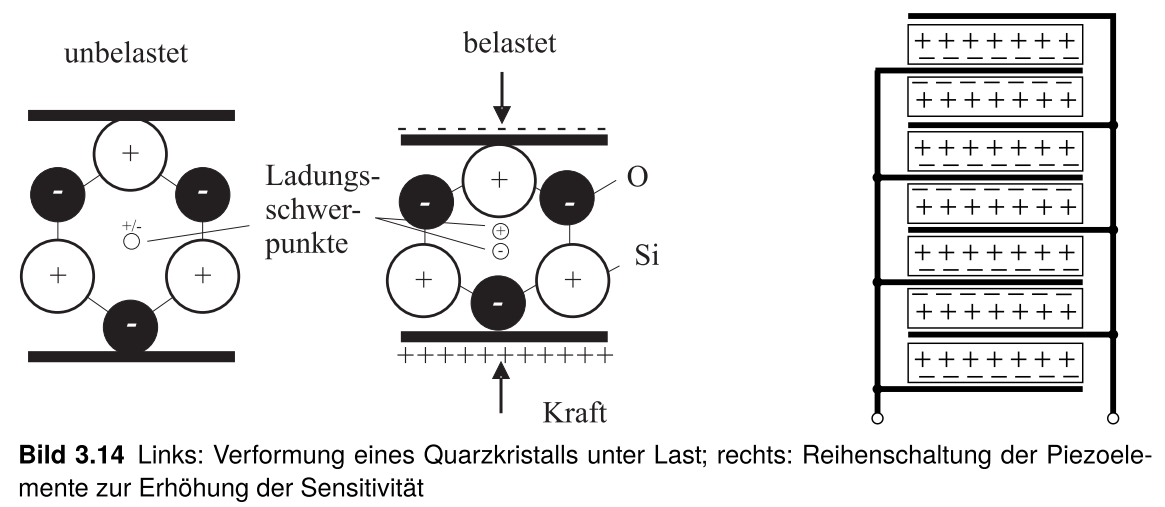
\includegraphics[width=\linewidth]{piezoelektrischerEffektquarz}
    \caption{Quarzkristall unter elastischer Verformung (\cite{Heimann.})}
  \end{subfigure}
  \begin{subfigure}[b]{0.45\linewidth}
    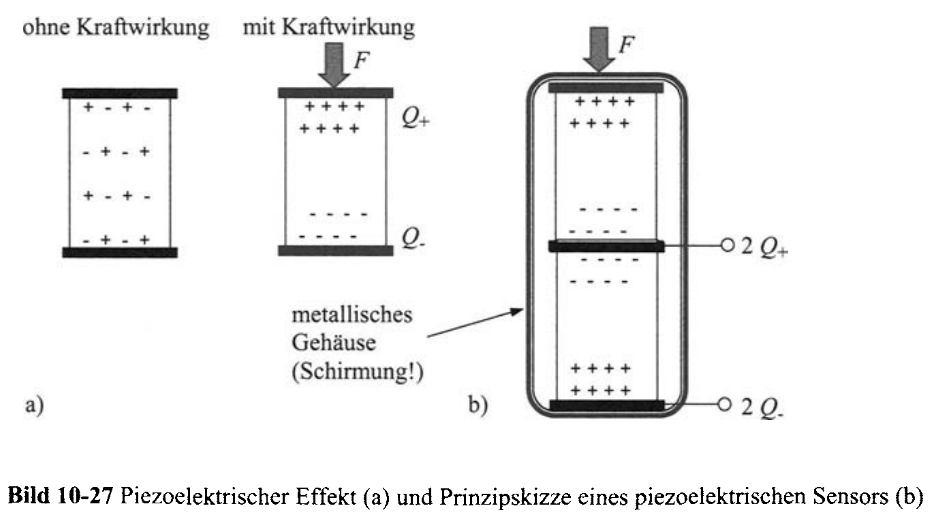
\includegraphics[width=\linewidth]{piezoelektrischerEffekt}
    \caption{Piezoelektrische Ladungsverformung an Materialien (\cite{Parthier.2006})}
  \end{subfigure}
  \caption{Piezoelektrischer Effekt mit Quarzstrukturverformung und Ladungsverteilung}
  \label{fig:piezoeffekt}
\end{figure}

Mit Gitterverschiebungen ist die Verteilung von Ionen in Quarzkristallstruktur verändert, führt zu eine Umwucht in Ladungschwerpunkt. Wo mehr Sauerstoffatomen sich befinden, ist negativ geladen und gleichzeitig an Siliziumseite positiv. Durch Reihenschaltung von Piezoelemente ist die Sensitivität erhöht. Auf dem rechten Bild gilt es für alle Piezoelemente, nicht nur Quarzkristalle. (\cite{Heimann.}, \cite{Parthier.2019})

Die Ladung wird durch die piezoelektrische Konstante und die Kraft bestimmt: 
\begin{center}
  $Q = k_{p} \cdot F$
\end{center}
Bei Quarz($SiO_2$) ist $k_p \approx 2,3 \cdot 10^{-12} As/N$ und bei Bariumtitanat(Keramik $BaTiO_3$) beträgt $k_p \approx 2,5 \cdot 10^{-10} As/N $

Piezoelemente wie PZT-5A haben gut Temperaturbeständigkeit und kann während hohe Schwankung an Temperatur konstante Leistung geben. Andere wie PZT-5H können nur in bestimmte Temperaturbereich verwendet werden, ist aber sehr empfindlich.

\begin{figure}[h!]
  \centering
  \label{fig:5h5a}
  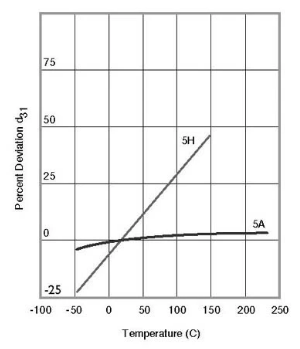
\includegraphics[width=0.5\textwidth]{5h5a}
  \caption{Vergleich Temperaturbeständigkeit zwischen PZT-5A und PZT-5H (\cite{PIEZO.COM.2021})}
\end{figure}

\subsubsection{Beispiel piezoelektrischer Drucksensor}

\begin{figure}[h!]
  \centering
  \label{fig:piezoelektrischedrucksensor}
  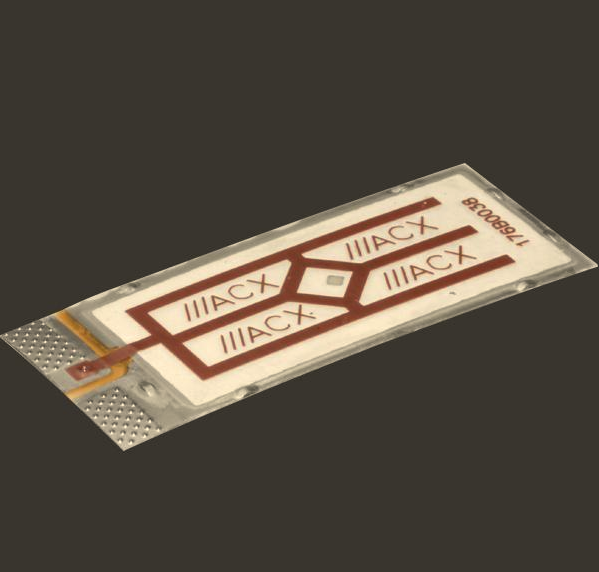
\includegraphics[width=0.65\textwidth]{piezoelektrischedrucksensor}
  \caption{Piezoelektrische Drucksensor PZT-5J (\cite{PIEZO.COM.2021})}
\end{figure}

Piezoelectric Bending Transducer is made from PZT-5J Material (Lead Zirconate Titanate), which is a compromise between PZT-5H and PZT-5A Material that is stable in mid range temperature. It can be operated from -60 to 120 grad celcius and has a capacity of 100nF.

\newpage
%% printbibliography
\printbibliography
\addcontentsline{toc}{section}{Literatur}
%% Umcomment these 4 lines to input \bibliography manually from other file
%% \newpage
%% \input{bibliography}
\begin{center}
\hyperref[sec:drucksensoren]{\large{$\uparrow$}}
\end{center}
\newpage
\pagestyle{fancy}
\textbf{Eigenständigkeitserklärung}

\vspace{6pt}

Hiermit versichere ich, dass ich den vorliegenden Bericht selbstständig und nur mit den angegebenen Hilfsmitteln verfasst habe. Alle Passagen, die ich wörtlich aus der Literatur oder aus anderen Quellen wie z. B. Internetseiten übernommen habe, habe ich deutlich als Zitat mit Angabe der Quelle kenntlich gemacht. 

\begin{flushright}
	\today

	
	Duy Nguyen
\end{flushright}

\addcontentsline{toc}{section}{Eigenständigkeitserklärung}
\end{document}
